\begin{comment}
- Gibs phenomenon
- Post-processing used (how impactful is removing non-distinct solutions?)
- How does clean TVD evolve with JVV steps (see proof)?
- Approximation ratio
- Numerical analysis (which mean to take)
\end{comment}

    \chapter{Résolution de problèmes \textsf{\#P}-difficile}

%-----------------------------------------------------------------------------%

\subsection*{Plan}

\begin{enumerate}
    \item Mentionner les problèmes étudiés
    \item Mentionner les méthodes utilisées (réseaux de tenseurs)
    \item Décrire les paramètres de l'étude (nombre d'instances, régimes de complexité, etc.)
    \item Expliquer les principaux résultats (compromis entre QAOA et GM-QAOA)
\end{enumerate}

\subsection*{Références}

%-----------------------------------------------------------------------------%

\section{Biais d'échantillonage des problèmes \textsf{\#P}-difficile}

\subsection*{Plan}

\begin{enumerate}
    \item Décrire le comportement de la non-uniformité pour les différents problèmes (ne pas oublier 2SAT)
\end{enumerate}

\subsection*{Références}

\begin{figure}[h]
    \centering
    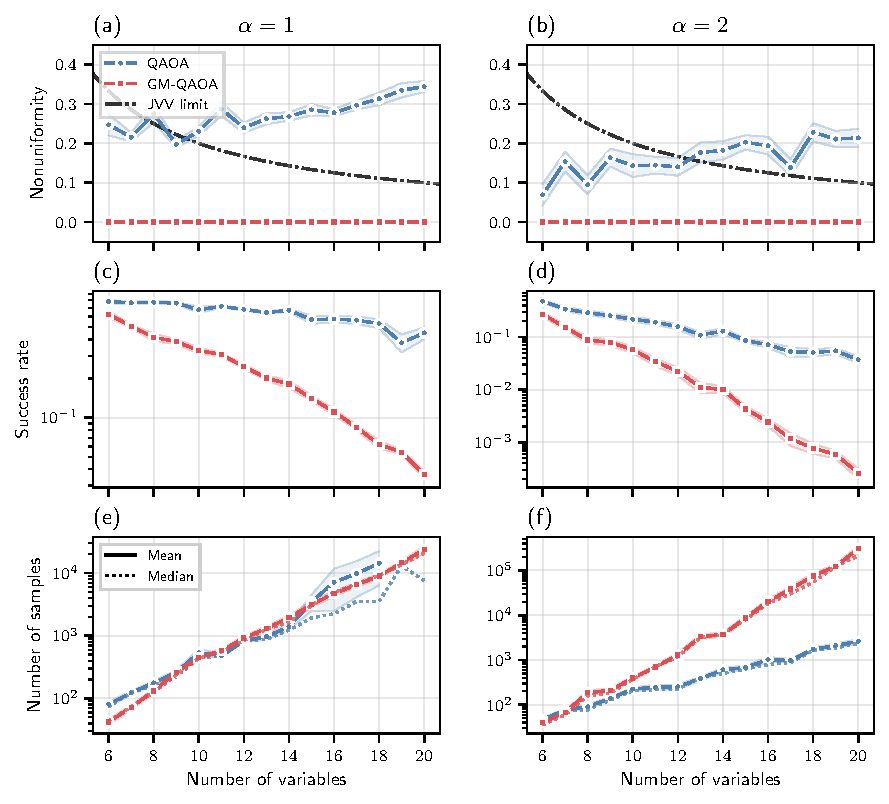
\includegraphics[width=1\textwidth]{figures/nae3sat-number-of-samples.pdf}
    \caption{}
    \label{fig:nae3sat-number-of-samples}
\end{figure}

\begin{figure}[h]
    \centering
    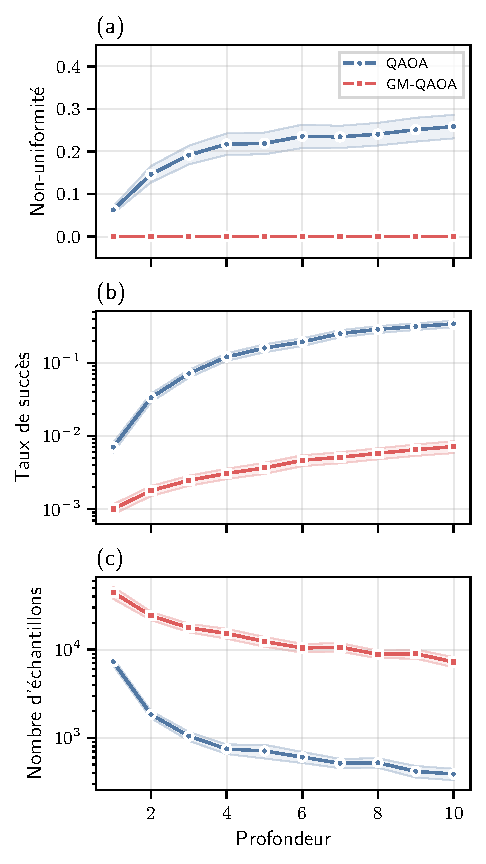
\includegraphics[width=0.5\textwidth]{figures/nae3sat-depth.pdf}
    \caption{}
    \label{fig:nae3sat-depth}
\end{figure}

\begin{figure}[h]
    \centering
    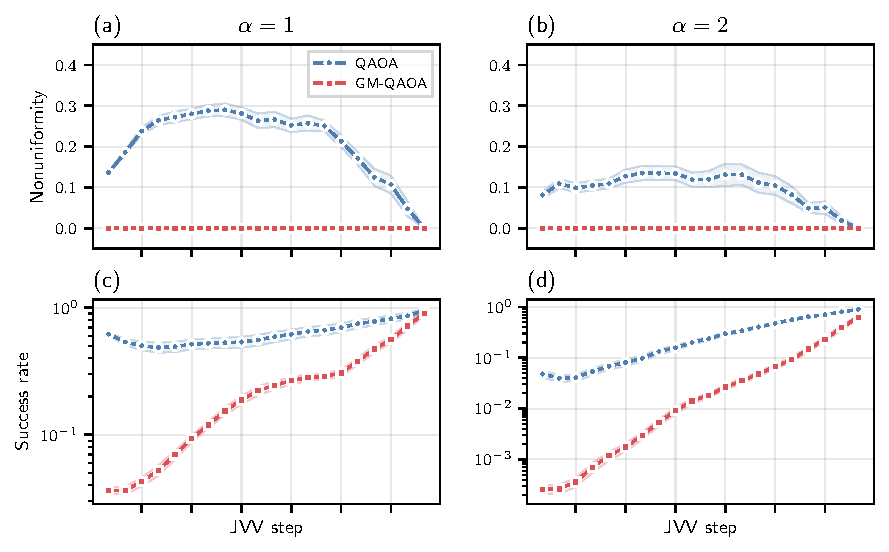
\includegraphics[width=1\textwidth]{figures/nae3sat-jvv-steps}
    \caption{}
    \label{fig:nae3sat-jvv-steps}
\end{figure}

%-----------------------------------------------------------------------------%


\section{Performance et comportement de l'algorithme VQCount}

\subsection*{Plan}

\begin{enumerate}
    \item  Décrire le taux de réussite et le nombre d'échantillons requis
    \item  Décrire la performance de l'algorithme en fonction de la profondeur du circuit
    \item Décrire l'efficacité d'échantillonage et la précision du compte
    \item Présenter brièvement le ratio d'approximation
\end{enumerate}

\subsection*{Références}

%-----------------------------------------------------------------------------%

\section{Transitions de phase observées par l'algorithme VQCount}

\subsection*{Plan}

\begin{enumerate}
    \item 
\end{enumerate}

\subsection*{Références}

%-----------------------------------------------------------------------------%
